\documentclass{article}\usepackage{graphicx, color}
%% maxwidth is the original width if it is less than linewidth
%% otherwise use linewidth (to make sure the graphics do not exceed the margin)
\makeatletter
\def\maxwidth{ %
  \ifdim\Gin@nat@width>\linewidth
    \linewidth
  \else
    \Gin@nat@width
  \fi
}
\makeatother

\definecolor{fgcolor}{rgb}{0.2, 0.2, 0.2}
\newcommand{\hlnumber}[1]{\textcolor[rgb]{0,0,0}{#1}}%
\newcommand{\hlfunctioncall}[1]{\textcolor[rgb]{0.501960784313725,0,0.329411764705882}{\textbf{#1}}}%
\newcommand{\hlstring}[1]{\textcolor[rgb]{0.6,0.6,1}{#1}}%
\newcommand{\hlkeyword}[1]{\textcolor[rgb]{0,0,0}{\textbf{#1}}}%
\newcommand{\hlargument}[1]{\textcolor[rgb]{0.690196078431373,0.250980392156863,0.0196078431372549}{#1}}%
\newcommand{\hlcomment}[1]{\textcolor[rgb]{0.180392156862745,0.6,0.341176470588235}{#1}}%
\newcommand{\hlroxygencomment}[1]{\textcolor[rgb]{0.43921568627451,0.47843137254902,0.701960784313725}{#1}}%
\newcommand{\hlformalargs}[1]{\textcolor[rgb]{0.690196078431373,0.250980392156863,0.0196078431372549}{#1}}%
\newcommand{\hleqformalargs}[1]{\textcolor[rgb]{0.690196078431373,0.250980392156863,0.0196078431372549}{#1}}%
\newcommand{\hlassignement}[1]{\textcolor[rgb]{0,0,0}{\textbf{#1}}}%
\newcommand{\hlpackage}[1]{\textcolor[rgb]{0.588235294117647,0.709803921568627,0.145098039215686}{#1}}%
\newcommand{\hlslot}[1]{\textit{#1}}%
\newcommand{\hlsymbol}[1]{\textcolor[rgb]{0,0,0}{#1}}%
\newcommand{\hlprompt}[1]{\textcolor[rgb]{0.2,0.2,0.2}{#1}}%

\usepackage{framed}
\makeatletter
\newenvironment{kframe}{%
 \def\at@end@of@kframe{}%
 \ifinner\ifhmode%
  \def\at@end@of@kframe{\end{minipage}}%
  \begin{minipage}{\columnwidth}%
 \fi\fi%
 \def\FrameCommand##1{\hskip\@totalleftmargin \hskip-\fboxsep
 \colorbox{shadecolor}{##1}\hskip-\fboxsep
     % There is no \\@totalrightmargin, so:
     \hskip-\linewidth \hskip-\@totalleftmargin \hskip\columnwidth}%
 \MakeFramed {\advance\hsize-\width
   \@totalleftmargin\z@ \linewidth\hsize
   \@setminipage}}%
 {\par\unskip\endMakeFramed%
 \at@end@of@kframe}
\makeatother

\definecolor{shadecolor}{rgb}{.97, .97, .97}
\definecolor{messagecolor}{rgb}{0, 0, 0}
\definecolor{warningcolor}{rgb}{1, 0, 1}
\definecolor{errorcolor}{rgb}{1, 0, 0}
\newenvironment{knitrout}{}{} % an empty environment to be redefined in TeX

\usepackage{alltt}
\usepackage[utf8]{inputenc}
\usepackage{graphicx}
\usepackage[colorlinks=true,urlcolor=blue]{hyperref}
\usepackage{array}
\usepackage{color}
\usepackage[english]{babel}
\usepackage{amsfonts}
\usepackage{url}
\usepackage{bm}
\usepackage[margin=2.5cm]{geometry}

\newcommand{\R}{\mathbb{R}}
\newcommand{\beq}{\begin{equation}}
\newcommand{\eeq}{\end{equation}}
\newcommand{\m}[1]{\mathbf{#1}}

\title{Spatial simulation code for 2014 EBV epidemic}
\author{Steven Riley}
\date{\today}

\sloppy
\hyphenpenalty 10000

%%%%%%%%%%%%%%%%%%%%%%%%%%%%%%%%%%%%%%%%%%%%%%%%%%
%%%%%%%%%%%%%%%%%%%%%%%%%%%%%%%%%%%%%%%%%%%%%%%%%%
%%%%%%%%%%%%%%%%%%%%%%%%%%%%%%%%%%%%%%%%%%%%%%%%%%
\IfFileExists{upquote.sty}{\usepackage{upquote}}{}
\begin{document}
\selectlanguage{english}

%% some knitr options



\maketitle




\newpage
%%%%%%%%%%%%%%%%%%%%%%%%%%%%%%%%%%%%%%%%%%%%%%%%%%
%%%%%%%%%%%%%%%%%%%%%%%%%%%%%%%%%%%%%%%%%%%%%%%%%%
%%%%%%%%%%%%%%%%%%%%%%%%%%%%%%%%%%%%%%%%%%%%%%%%%%

%%%%%%%%%%%%%%%%%%%%%%%%%%
%%%%%%%%%%%%%%%%%%%%%%%%%%
%%%%%%%%%%%%%%%%%%%%%%%%%%
%%%%%%%%%%%%%%%%%%%%%%%%%%

This R script goes with a bacth file in the testsuite directory of the
id\_sptail\_sim library. After grabbing the code as a zip file from
http:XXgoo.glXabcdef, you should be able to generate the simulation
results and then the pdf of this script with the following commands

\begin{verbatim}
gunzip id_spatial_sim.zip 
cd id_spatial_sim/g++ 
make 
cd ../testsuite 
./fast_test.sh 
\end{verbatim}


When this is not being run in bacth mode, we need to set the working directory.
This appears here as a comment, so it is not run when in batch mode.

\begin{knitrout}
\definecolor{shadecolor}{rgb}{0.969, 0.969, 0.969}\color{fgcolor}\begin{kframe}
\begin{alltt}
\hlfunctioncall{rm}(list=\hlfunctioncall{ls}(all=TRUE))
\hlcomment{# setwd("~/Dropbox/git/id_spatial_sim/testsuite")}
\end{alltt}
\end{kframe}
\end{knitrout}


First we declare some packages and local libraries that might be needed. If the
script goes into more general use, the dependency on the local libraries will
have to be removed.

\begin{knitrout}
\definecolor{shadecolor}{rgb}{0.969, 0.969, 0.969}\color{fgcolor}\begin{kframe}
\begin{alltt}
\hlfunctioncall{require}(\hlstring{"raster"})
\end{alltt}


{\ttfamily\noindent\itshape\color{messagecolor}{\#\# Loading required package: raster}}

{\ttfamily\noindent\itshape\color{messagecolor}{\#\# Loading required package: methods}}

{\ttfamily\noindent\itshape\color{messagecolor}{\#\# Loading required package: sp}}\begin{alltt}
\hlfunctioncall{require}(\hlstring{"scales"})
\end{alltt}


{\ttfamily\noindent\itshape\color{messagecolor}{\#\# Loading required package: scales}}\begin{alltt}
\hlfunctioncall{require}(\hlstring{"sp"})
\hlfunctioncall{require}(\hlstring{"rgdal"})
\end{alltt}


{\ttfamily\noindent\itshape\color{messagecolor}{\#\# Loading required package: rgdal}}

{\ttfamily\noindent\itshape\color{messagecolor}{\#\# rgdal: version: 0.8-9, (SVN revision 470)\\\#\# Geospatial Data Abstraction Library extensions to R successfully loaded\\\#\# Loaded GDAL runtime: GDAL 1.9.2, released 2012/10/08\\\#\# Path to GDAL shared files: /Library/Frameworks/R.framework/Versions/3.0/Resources/library/rgdal/gdal\\\#\# Loaded PROJ.4 runtime: Rel. 4.8.0, 6 March 2012, [PJ\_VERSION: 480]\\\#\# Path to PROJ.4 shared files: /Library/Frameworks/R.framework/Versions/3.0/Resources/library/rgdal/proj}}\begin{alltt}
\hlfunctioncall{source}(\hlstring{"~/Dropbox/svneclipse/idsource/R/stevensRfunctions.R"})
\end{alltt}
\begin{verbatim}
## Reading in stevensRfunctions.R
## The latest version of this file can be loaded into R with
## source("http://idsource.googlecode.com/svn/trunk/R/stevensRfunctions.R") or
## source("http://tinyurl.com/5t7gwnv")
## Revision X of this file can be loaded into R with
## source("http://idsource.googlecode.com/svn-history/rX/trunk/R/stevensRfunctions.R")
\end{verbatim}
\end{kframe}
\end{knitrout}


The first line of the batch file builds a synthetic population with density
proportional the ebola affected region in west Africa, but much smaller. With a total population of only
100,000. Each person has, one average, 10 network links but these links are
distributed entirely randomly in space. This takes a while because the
average population is very low and there is high variability. Hence the
accept-reject method for assinging nodes has many rejection steps. We assume
that only one individual lives in a household for this population. 

%% <<>>=
%% # system("../g++/ebola_build.exe ./params/fast_test_build_params.in ./output/small_pop1")  
%% @

The second line of the batch file runs an outbreak of only two generations 20
times. The outbreak is seeded in the same area as the reported patient zero for
the 2014 Ebola outbreak. There are 4 iniitally infectious individuals at time
$t=0$. Transmission is only via the spatial kernel and thus allows us to test
that the basic reproductive number is parameterized correctly. We can also
report the serial interval. 

%{\bf Table 1. Key parameters of the simulation model}
%
%\begin{tabular}{lll} \hline
%Parameter & Value & Notes \\ \hline
%$R_0$ spatial & 1.6 & From fully spatial kernel \\
%Mean latent period & XXX & XXX \\ \hline
%\end{tabular}

We first load the linelist of events from all the realizations. And check the
dimensions of the output. The output was designed before csvs became so
dominant!

\begin{knitrout}
\definecolor{shadecolor}{rgb}{0.969, 0.969, 0.969}\color{fgcolor}\begin{kframe}
\begin{alltt}
dat0 <- \hlfunctioncall{read.table}(file=\hlstring{"./output/ft_sp_pset_0_Events.out"},header=TRUE)
dimDat0 <- \hlfunctioncall{dim}(dat0)
noevents <- dimDat0[1]
nocols <- dimDat0[2]
\end{alltt}
\end{kframe}
\end{knitrout}


The column headings describe the information captured in the event file
\begin{knitrout}
\definecolor{shadecolor}{rgb}{0.969, 0.969, 0.969}\color{fgcolor}\begin{kframe}
\begin{alltt}
\hlfunctioncall{names}(dat0)
\end{alltt}
\begin{verbatim}
##  [1] "Run"        "Day"        "Event"      "Index"      "X"         
##  [6] "Y"          "Generation" "infector"   "infect_x"   "infect_y"
\end{verbatim}
\end{kframe}
\end{knitrout}


We can subset these 'data' to look at only infection. Then examine the number of
infections by generation for each realization.

\begin{knitrout}
\definecolor{shadecolor}{rgb}{0.969, 0.969, 0.969}\color{fgcolor}\begin{kframe}
\begin{alltt}
tabInfs0 <- dat0[dat0$Event==0,]
\hlfunctioncall{table}(tabInfs0$Run,tabInfs0$Generation)
\end{alltt}
\begin{verbatim}
##    
##      1  2
##   0  4  5
##   1  4  0
##   2  4  5
##   3  4 12
##   4  4  8
##   5  4  8
##   6  4 11
##   7  4 14
##   8  4 11
##   9  4  2
\end{verbatim}
\end{kframe}
\end{knitrout}


And look at the average number in the second generation divided by the number of
seeds as a test of the $R_0$ parameterization. 

\begin{knitrout}
\definecolor{shadecolor}{rgb}{0.969, 0.969, 0.969}\color{fgcolor}\begin{kframe}
\begin{alltt}
\hlfunctioncall{table}(tabInfs0$Generation)[2]/\hlfunctioncall{table}(tabInfs0$Generation)[1]
\end{alltt}
\begin{verbatim}
##   2 
## 1.9
\end{verbatim}
\end{kframe}
\end{knitrout}


Its difficult to tell if this is accurate with such small numbers, so we can
load up the similar run with 100 realisations.

\begin{knitrout}
\definecolor{shadecolor}{rgb}{0.969, 0.969, 0.969}\color{fgcolor}\begin{kframe}
\begin{alltt}
dat1 <- \hlfunctioncall{read.table}(file=\hlstring{"./output/ft_sp_pset_1_Events.out"},header=TRUE)
\hlfunctioncall{dim}(dat1)
\end{alltt}
\begin{verbatim}
## [1] 4264   10
\end{verbatim}
\begin{alltt}
tabInfs1 <- dat1[dat1$Event==0,]
estR0 <- \hlfunctioncall{table}(tabInfs1$Generation)[2] / \hlfunctioncall{table}(tabInfs1$Generation)[1]
estR0
\end{alltt}
\begin{verbatim}
##     2 
## 1.665
\end{verbatim}
\end{kframe}
\end{knitrout}


Might also be worth looking at the distribution of the ratio of secondary cases
for each realization. So we make a table of generations by run and plot a
histogram of the ratios for each realization. You can see quite a bit of
variance in the size of the second generation of this model. Note that the
offspring distribution will be even more highly over-dispersed because these
results are based on a seed of 4.

\begin{knitrout}
\definecolor{shadecolor}{rgb}{0.969, 0.969, 0.969}\color{fgcolor}\begin{kframe}
\begin{alltt}
tabRunGen1 <- \hlfunctioncall{table}(tabInfs1$Run,tabInfs1$Generation)
\hlfunctioncall{hist}( tabRunGen1[,2]/tabRunGen1[,1],breaks=\hlfunctioncall{seq}(0,7,0.25),
      xlab=\hlstring{"Ratio first to second gens"},main=\hlstring{""})
\hlfunctioncall{abline}(v=estR0,lwd=2,col=\hlstring{"red"})	
\end{alltt}
\end{kframe}

{\centering 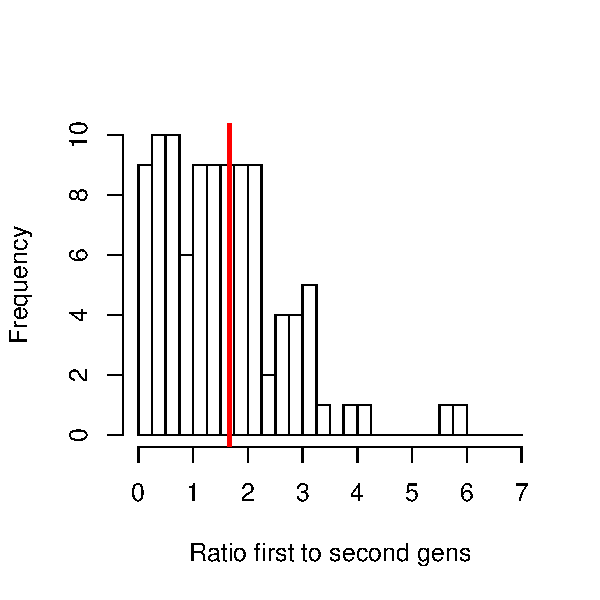
\includegraphics[width=\textwidth]{figs/unnamed-chunk-10} 

}



\end{knitrout}


It is also straightforward to look at the distributions of different waiting
times in the model because we 'observe' them directly in this idealized
linelist. So the average serial interval is equal to the average time of the
infection event in the second generation.

\begin{knitrout}
\definecolor{shadecolor}{rgb}{0.969, 0.969, 0.969}\color{fgcolor}\begin{kframe}
\begin{alltt}
vecTimesG1 <- tabInfs1[tabInfs1$Generation==2,\hlstring{"Day"}] 
\hlfunctioncall{mean}(vecTimesG1)
\end{alltt}
\begin{verbatim}
## [1] 16.51
\end{verbatim}
\begin{alltt}
\hlfunctioncall{hist}(vecTimesG1,breaks=\hlfunctioncall{seq}(0,50,2),main=\hlstring{""},
    xlab=\hlstring{"Time from exposure to \hlfunctioncall{infection} (2 day bins)"})
\end{alltt}
\end{kframe}

{\centering 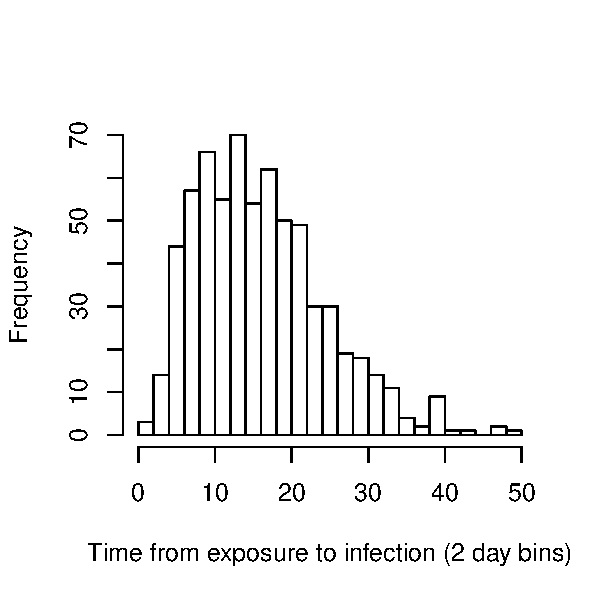
\includegraphics[width=\textwidth]{figs/unnamed-chunk-11} 

}



\end{knitrout}


Its a highly over-dospersed distribution, suggesting that events such as the
long time from exposure to infection for the non-African infection event
in Spain are not entirely inconsistent with the NEJM estimated parameters.

\subsection{Spatial analysis}

Next we load up the population desity on which the model was based and look at
the spatial distribution of these initial infections. The simulation is using
the kernel shape and parameters from the SI file that Azra sent last week.

Note that the pattern is way too diffuse because the population
density is only at about 1\% of the real density. The same kernel will bring
all these first generation events in much closer with the real population
density. This section is working, but I can't get the aggregate function to work
properly and give lower resolution for the event map.

\begin{knitrout}
\definecolor{shadecolor}{rgb}{0.969, 0.969, 0.969}\color{fgcolor}\begin{kframe}
\begin{alltt}
popgrid <- \hlfunctioncall{read.asciigrid}(\hlstring{"../data/westAfricaAscii_agg100.asc"},as.image=TRUE)
\hlfunctioncall{sum}(popgrid$z,na.rm=TRUE)
\end{alltt}
\begin{verbatim}
## [1] 24881385
\end{verbatim}
\begin{alltt}
popgrid$x <- popgrid$x * pi / 180
popgrid$y <- popgrid$y * pi / 180
epiImage <- \hlfunctioncall{eventImage}(dat1,popgrid,0,0,1000,0,1000)
\hlfunctioncall{image}(popgrid$x,popgrid$y,\hlfunctioncall{log}(popgrid$z+0.5),col=\hlfunctioncall{rev}(\hlfunctioncall{grey_pal}()(100)),xlab=\hlstring{""},ylab=\hlstring{""})
\hlfunctioncall{image}(epiImage$x,epiImage$y,epiImage$z,add=TRUE)
\end{alltt}
\end{kframe}

{\centering 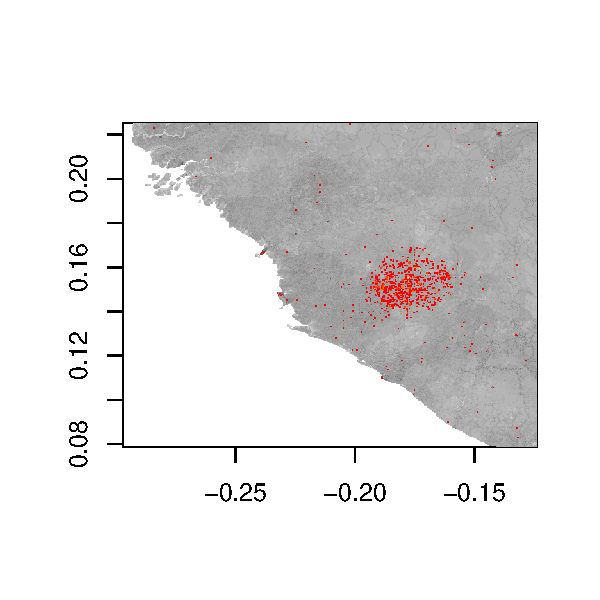
\includegraphics[width=\textwidth]{figs/unnamed-chunk-12} 

}



\end{knitrout}


Next is to figure out how to extract district incidence from the simulation
results so it can be compared with the data.

\begin{knitrout}
\definecolor{shadecolor}{rgb}{0.969, 0.969, 0.969}\color{fgcolor}\begin{kframe}
\begin{alltt}
shapeDir <- \hlstring{"/Users/sriley/srileytmp/sfs"}
dists <- \hlfunctioncall{readOGR}(dsn=shapeDir,layer=\hlstring{"ThreeCountries"})
\end{alltt}
\begin{verbatim}
## OGR data source with driver: ESRI Shapefile 
## Source: "/Users/sriley/srileytmp/sfs", layer: "ThreeCountries"
## with 67 features and 28 fields
## Feature type: wkbPolygon with 2 dimensions
\end{verbatim}
\begin{alltt}
\hlfunctioncall{summary}(dists)
\end{alltt}
\begin{verbatim}
## Object of class SpatialPolygonsDataFrame
## Coordinates:
##       min    max
## x -15.081 -7.367
## y   4.343 12.677
## Is projected: FALSE 
## proj4string :
## [+proj=longlat +datum=WGS84 +no_defs +ellps=WGS84 +towgs84=0,0,0]
## Data attributes:
##     OBJECTID    WHO_REGION ISO_2_CODE   ADM2_NAME       ADM1_NAME 
##  Min.   : 422   AFRO:67    GN:38      BEYLA  : 1   N'ZEREKORE: 6  
##  1st Qu.:1028              LR:15      BO     : 1   BOKE      : 5  
##  Median :1724              SL:14      BOFFA  : 1   CONAKRY   : 5  
##  Mean   :1726                         BOKE   : 1   KANKAN    : 5  
##  3rd Qu.:2235                         BOMBALI: 1   KINDIA    : 5  
##  Max.   :3439                         BOMI   : 1   LABE      : 5  
##                                       (Other):61   (Other)   :36  
##         ADM0_NAME                 ADM2_CODE                 ADM1_CODE 
##  GUINEA      :38   GN001001001000000000: 1   GN001008000000000000: 6  
##  LIBERIA     :15   GN001001002000000000: 1   GN001001000000000000: 5  
##  SIERRA LEONE:14   GN001001003000000000: 1   GN001002000000000000: 5  
##                    GN001001004000000000: 1   GN001004000000000000: 5  
##                    GN001001005000000000: 1   GN001005000000000000: 5  
##                    GN001002001000000000: 1   GN001006000000000000: 5  
##                    (Other)             :61   (Other)             :36  
##                 ADM0_CODE       STARTDATE        ENDDATE  
##  GN001000000000000000:38   2000/01/01:67   9999/12/31:67  
##  LR001000000000000000:15                                  
##  SL001000000000000000:14                                  
##                                                           
##                                                           
##                                                           
##                                                           
##                                      GUID    ISO_3_CODE WHO_CODE ADM2_ALTNA
##  {02B44F7F-85C2-4177-B4C6-0D058ABA7D8E}: 1   GIN:38     GUI:38   NA's:67   
##  {0FEF85C0-C239-40FD-A0BB-4844FDA4D6F9}: 1   LBR:15     LIB:15             
##  {10025130-AD44-4B4F-A231-45BBE541B861}: 1   SLE:14     SIL:14             
##  {16FAC340-B054-43D4-9089-E51664302A43}: 1                                 
##  {1ACFF5CE-8BE8-41AD-8B75-23006FA2D9E8}: 1                                 
##  {2028113B-9DAE-49D0-AB36-0F00F4E3D4C1}: 1                                 
##  (Other)                               :61                                 
##  ADM2_ALTCO     ISO_2_ADM2      LVL           WHO_STATUS    UN_CODE   
##  NA's:67    GN_BEYLA : 1   Min.   :2   Member state:67   Min.   :324  
##             GN_BOFFA : 1   1st Qu.:2                     1st Qu.:324  
##             GN_BOKE  : 1   Median :2                     Median :324  
##             GN_COYAH : 1   Mean   :2                     Mean   :425  
##             GN_DABOLA: 1   3rd Qu.:2                     3rd Qu.:430  
##             GN_DALABA: 1   Max.   :2                     Max.   :694  
##             (Other)  :61                                              
##  UNICEF_REG   CENTER_LON       CENTER_LAT   
##  WCARO:67   Min.   :-14.36   Min.   : 4.75  
##             1st Qu.:-12.79   1st Qu.: 7.73  
##             Median :-11.35   Median : 9.24  
##             Mean   :-11.24   Mean   : 8.96  
##             3rd Qu.: -9.76   3rd Qu.:10.50  
##             Max.   : -7.85   Max.   :12.38  
##                                             
##                                    GlobalID    SHAPE_Leng      SHAPE_Area    
##  {003C987E-55FF-4142-B1A4-FBB9AEB9B470}: 1   Min.   :0.188   Min.   :0.0015  
##  {016CAA15-BF3B-46B0-A410-21EACE8F161F}: 1   1st Qu.:2.772   1st Qu.:0.2600  
##  {02D83A72-0004-4280-AC2C-A9EB65DFFC3E}: 1   Median :3.587   Median :0.4444  
##  {0607C700-9B3B-43FA-9109-969CCF8C59A0}: 1   Mean   :3.636   Mean   :0.5081  
##  {0719C492-5BCA-4CF4-B354-7C041EFCE375}: 1   3rd Qu.:4.795   3rd Qu.:0.7024  
##  {0AECF59E-1559-4D1F-9854-2F2A7ACD8803}: 1   Max.   :8.021   Max.   :1.4793  
##  (Other)                               :61                                   
##       ADM1_VIZ_N   ADM2_VIZ_N
##  N'Zerekore: 6   Beyla  : 1  
##  Boke      : 5   Bo     : 1  
##  Conakry   : 5   Boffa  : 1  
##  Kankan    : 5   Boke   : 1  
##  Kindia    : 5   Bombali: 1  
##  Labe      : 5   Bomi   : 1  
##  (Other)   :36   (Other):61
\end{verbatim}
\begin{alltt}
\hlfunctioncall{plot}(dists)
\end{alltt}
\end{kframe}

{\centering 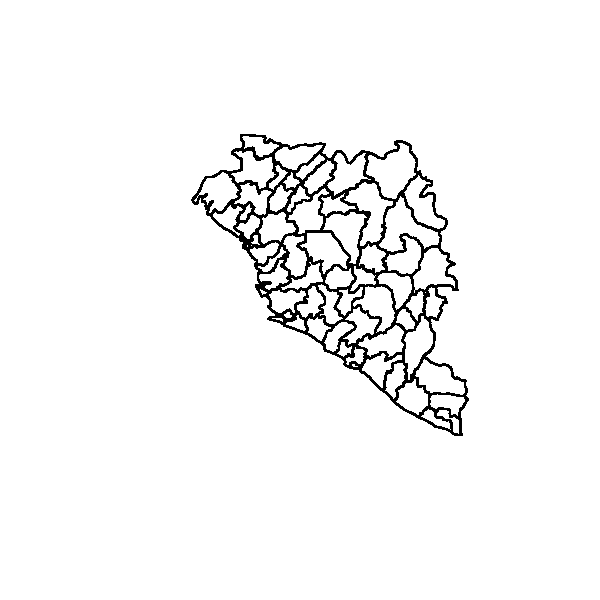
\includegraphics[width=\textwidth]{figs/unnamed-chunk-13} 

}



\end{knitrout}


\end{document}

